\chapter{Background knowledge}
\section{Gaussian Mixture Model (GMM)}
Gaussian Mixture Model (GMM) is a probability model, which is a extension of Gaussian distribution, widely used in many machine learning related field, such as speech recognition, image recognition, video search, etc. 

A GMM is a weighted sum of $M$ gaussian density function, which is given by the following form:
\begin{equation}
p(\mathbf{x}|\mathbf{\Theta}) = \sum_{i = 0}^{M - 1} c_iN(\mathbf{x}|\mathbf{\mu}_i, \mathbf{\Sigma}_i),
\end{equation}
where $\mathbf{x}$ is an $D$ dimensions variable, $\Theta$ is parameter of GMM, including $\mathbf{c}$, $\mathbf{\mu}$ and $\mathbf{\Sigma}$. $c_i$ is the weight of $i^{th}$ mixture, satisfy the following constraint:
\begin{equation}
\sum_{i=0}^{M-1}c_i=1,
\end{equation}
while $\mathbf{\mu}_i$ and $\mathbf{\Sigma}_i$ are the mean vector and covariance matrix, respectively. $N(\mathbf{x}|\mathbf{\mu}_i, \mathbf{\Sigma}_i), i = 0, 1, .., M - 1$, is the gaussian density function, i.e.
\begin{equation}
 N(\mathbf{x}|\mathbf{\mu}_i, \mathbf{\Sigma}_i) = \frac{1}{\sqrt{(2\pi)^D|\mathbf{\Sigma}_i|}}e^{-\frac{1}{2}(\mathbf{x}-\mathbf{\mu}_i)^T\mathbf{\Sigma}_i^{-1}(\mathbf{x}-\mathbf{\mu}_i)}.
\end{equation}

In practice, in order to reduce the complexity of calculation, for covariance matrix $\Sigma$, we usually use diagonal matrix instead of full covariance matrix, which means we regard $D$ dimensions of variable $\mathbf{x}$ to be independent. Then we have
\begin{equation}
p(\mathbf{x}|\mathbf{\Theta}) = \sum_{i = 0}^{M - 1} c_i\prod_{d=0}^{D-1} \frac{1}{\sqrt{(2\pi)}\sigma_{id}}e^{-\frac{1}{2\sigma_{id}^{2}}(x_d-\mu_{id})^2},\label{GMM-p}
\end{equation}
where $\mu_{id}$ and $\sigma_{id}$ are the mean and standard deviation of demension $d$ of mixtrue $i$.
\section{Hidden Markov Model (HMM)}
Hidden Markov Model is a statistical model, which assuming the system to be modeled as a Markov process with hidden states. Like GMM, HMM is also widely used in speech recognition, audio processing, etc.

In practice, audio signal usually be modeled as a {\em left-to-right} HMM. {\em Left-to-right} here means that the transitions are not allowed from right to left. The following graph shows a 5-state left-to-right HMM. Since the input (observation) values are continuous in audio processing (CHMM), we usually use a GMM to model each states.
\begin{figure}[!h]
\centering
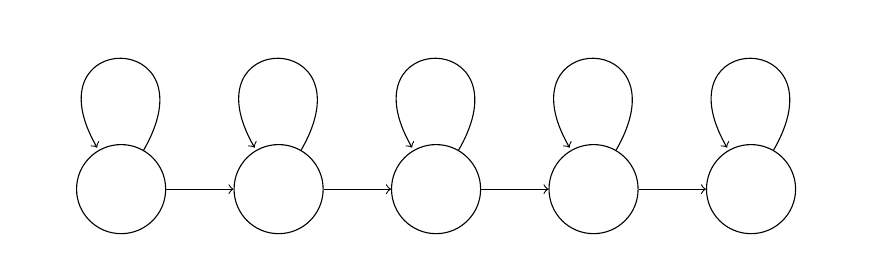
\begin{tikzpicture}
\tikzstyle{every node}=[circle, color=black, draw, inner sep=0.4cm]
\draw (-4, 0) node (A) {} edge [in=120,out=60,loop,->]();
\draw (-2, 0) node (B) {} edge [in=120,out=60,loop,->]();
\draw (0, 0) node (C) {} edge [in=120,out=60,loop,->]();
\draw (2, 0) node (D) {} edge [in=120,out=60,loop,->]();
\draw (4, 0) node (E) {} edge [in=120,out=60,loop,->]();
\draw[->] (A) -- (B);
\draw[->] (B) -- (C);
\draw[->] (C) -- (D);
\draw[->] (D) -- (E);
\end{tikzpicture}
\caption{A 5-state left-to-right HMM}
\end{figure}

Formally, a CHMM can be described as $\lambda = \lambda(N_s, N_m, N_d, \pi, A, B)$, where $N_s$ is the number of hidden states, $N_m$ is the number of mixtures of GMM in each states\footnote{Usually, the number of mixtures of each state are the same.}, $N_d$ is the number of dimensions of observation/input data. 

$\pi = (\pi_0, \pi_1, \ldots, \pi_{N_s - 1})$ is probability vector of initial states, i.e.
\begin{equation}
\pi_i = p(q_0=state_i),
\end{equation}
where $q_t$ is the state of time $t$.

$A = (a_{ij})$ is an $N_s * N_s$ matrix, which is called transition matrix. $a_{ij}$ stands for the probability of transition from state $i$ to state $j$, i.e.
\begin{equation}
a_{ij} = p(q_{t + 1} = state_j|q_t = state_i).
\end{equation}

$B = {b_0, b_1,\cdots b_{N_s -1}}$ are gaussian mixture functions, where $b_i$ is the gaussian mixture function of state $i$, \ie
\begin{equation}
b_i = p(\mathbf{x}|\mathbf{\Theta_{state_i}})
\end{equation}
\section{Knowledge base}
Knowledge base is a database used to store large and complex data. There are many knowledge bases built by researchers. In this section, we will introduce some of them.
\subsection{Probase}
Probase \cite{wu2012probase}\footnote{http://research.microsoft.com/en-us/projects/probase} is a probabilistic taxonomy for text understanding, built by Microsort. The core taxonomy of Probase (Probase v5.2) contains more than 2.7 million concepts, connected by the concept-entity relations. There is a frequency between each concept-entity pair in Probase. For example, given {\em google} and {\em company}, there is a $f(I=google|C=company)$, which indicates the frequency people refer to {\em google} when they say {\em company}. Table \ref{tab:pro} shows an example of some hyponyms of {\em instrument}.
\begin{table}[!htb]
\centering
\begin{tabular}{llll}
\hline
concept & entity & frequency & popularity\\\hline
instrument & guitar & 768 & 586\\
instrument & piano & 635 & 474\\
instrument & violin & 475 & 395\\
instrument & drum & 420 & 299\\
instrument & flute & 367 & 316\\
instrument & bass & 201 & 148\\
instrument & keyboard & 193 & 146\\
instrument & saxophone & 182 & 162\\
instrument & clarinet & 170 & 144\\
instrument & cello & 163 & 145\\
instrument & trumpet & 156 & 132\\
instrument & mandolin & 143 & 117\\
instrument & banjo & 131 & 114\\
instrument & harp & 131 & 117\\
instrument & trombone & 96 & 84\\
instrument & accordion & 91 & 88\\
instrument & percussion & 90 & 86\\
instrument & tuba & 89 & 60\\
instrument & oboe & 88 & 80\\
instrument & harmonica & 83 & 78\\\hline
\end{tabular}
\caption{An example of some hyponyms of {\em instrument}}
\label{tab:pro}
\end{table}
\subsection{WordNet}
WordNet \cite{miller1995wordNet}\footnote{http://wordnet.princeton.edu} is a large English lexical database created and maintained by the {\em Cognitive Science Laboratory} of {\em Princeton University}. It contains nouns, verbs, adjectives and adverbs, and groups them into synonyms sets (synsets), each express a distinct concept. Also, there are some relations between synsets recorded in WordNet, such as {\em is-a relation}, {\em part-of relation}, {\em made-of relation}, etc. Figure \ref{fig:wn} shows a example of relation in WordNet. The word ``activity'' has hyponym ``job'', and ``job'' has hyponym ``sport'' and ``career'', etc. Also, we can know that ``business'', ``line of work'', ``line'', ``occupation'' and ``job'' form a synset.

\begin{figure}[!hb]
\centering
\includegraphics[width=0.8\textwidth]{figures/wordnet.eps}
\caption{Example of relation in WordNet}
\label{fig:wn}
\end{figure}

\section{Stanford NLP}
Stanford NLP \cite{toutanovastanford,stanfordtoolkits} is a tool developed by Stanford Natural Language Processing Group, which aims to allow computers to understand and process human languages. It can do many of NLP-related works such as {\em POS tagging}, {\em lemmatization}, {\em sentence splitting}, {\em name entity recognition (NER)}, {\em sentence-level dependency analysis}, etc. Table \ref{tab:res} and figure \ref{fig:res} show the results of analyzing sentence {\em ``Ann first found success with the release of her second studio album.''}.
\begin{table}[!htb]
\centering
\begin{tabular}{lll}
\hline
Word & Lemmatization & POS tagging\\\hline
Ann & Ann & NNP (proper noun, singular)\\
first & first & RB (adverb)\\
found & find & VBD (verb, past tense)\\
success & success & NN (noun, singular or mass)\\
with & with & IN (preposition or subordinating conjunctior)\\
the & the & DT (determiner)\\
release & release & NN (noun, singular or mass)\\
of & of & IN (preposition or subordinating conjunctior)\\
her & she & PRP\$ (possessive pronoun)\\
second & second & JJ (adjective)\\
studio & studio & NN (noun, singular or mass)\\
album & album & NN (noun, singular or mass)\\\hline
\end{tabular}
\caption{An example of lemmatization and POS tagging}
\label{tab:res}
\end{table}

\begin{figure}
\centering
\includegraphics[width=0.8\textwidth]{figures/nlp.eps}
\caption{An example of sentence-level dependency analysis}
\label{fig:res}
\end{figure}

\section{Kullback-Leibler divergence}
Kullback-Leibler (KL) divergence is a measure of the difference between two probability distributions. More precisely, KL divergence of $Q$ from $P$, denoted by $KL(P||Q)$, is a measure of the information loss when we use $Q$ to approximate $P$.

For continuous random variables $\mathbf{x}$ and two distributions $P$ and $Q$, the KL divergence of $Q$ from $P$ is defined as:
\begin{equation}
KL(P||Q) = \int_{-\infty}^{+\infty}\ln(\frac{p(\mathbf{x})}{q(\mathbf{x})})p(\mathbf{x})\mathrm{d}x,
\label{eq:kl}
\end{equation}
where $p(\mathbf{x})$ and $q(\mathbf{x})$ are the density functions of $P$ and $Q$.

From the above equation, we can find that KL divergence is non-symmetric \ie $KL(P||Q)$ may not equal to $KL(Q||P)$. In practice, sometimes a symmetric measure is needed, thus $\overline{KL}(P||Q)$ is often used, that is:
\begin{equation}
\overline{KL}(P||Q) = \overline{KL}(Q||P) = \frac{1}{2}(KL(P||Q) + KL(Q||P)).
\end{equation}
